\laborator{Решение дифференциальных уравнений}

\goal ознакомиться с возможностями математического пакета Mathcad при решении дифференциальных уравнений в различных вариантах постановки задачи (задача Коши, краевая задача).

\subsubsection*{Теория}

Дифференциальные уравнения позволяют выразить соотношения между изменениями физических величин, и потому они имеют большое значение в прикладных задачах. Обыкновенным дифференциальным уравнением порядка $r$ называется уравнение:
\begin{equation} \label{dif.mdif}
F(x,y(x),y^\prime(x),y^{\prime \prime}(x), ... , y^r(x))=0,
\end{equation}
которое связывает независимую переменную $x$, искомую функцию и ее производные. Решение дифференциального уравнения \ref{dif.mdif} заключается в отыскании функций, которые удовлетворяют этому уравнению для всех значений в определенном конечном или бесконечном интервале. Решения могут быть проверены подстановкой в уравнение \ref{dif.mdif}.

Общее решение обыкновенного дифференциального уравнения порядка $r$ имеет вид:
\begin{equation}
y=y(x,C_1,C_2, ... ,C_r),
\end{equation}
где $С_1$, $С_2$, ... , $С_r$ --- произвольные постоянные (постоянные интегрирования). Каждый частный выбор этих постоянных дает частное решение. В задаче Коши (начальной задаче) требуется найти частное решение, удовлетворяющее $r$ начальным условиям:
\begin{equation}
y(x_0)=y_0, \newline
y^{\prime}(x_0)=y_0^{\prime}, ... , y^{r}(x_0)=y^r_0,
\end{equation}
по которым определяются $r$ постоянных $С_1$, $С_2$, ... , $С_r$. В краевой задаче на функцию $y(x)$ и ее производные накладываются $r$ краевых условий в точках $x=a$ и $x=b$, то есть условия накладываются на разных границах.

Методы численного решения обыкновенных дифференциальных уравнений в форме задачи Коши разработаны досконально \cite{shipachevvs2005}. Самыми распространенными из них являются алгоритмы Рунге~-- Кутта, успешно используемые для решения подавляющего большинства дифференциальных уравнений. 

В Mathcad имеются специальные встроенные функции, позволяющие находить решения как линейных, так и нелинейных систем дифференциальных уравнений. Несмотря на различные методы поиска решения, каждая из этих функций требует, чтобы были заданы, по крайней мере, следующие величины, необходимые для поиска решения:
\begin{itemize}
	\item начальные условия; 
	\item набор точек, в которых нужно найти решение;
	\item само дифференциальное уравнение, записанное в некотором специальном виде.
\end{itemize}

Для решения дифференциальных уравнений и систем дифференциальных уравнений в Mathcad есть функция \mc{ rkfixed(у0, t0, t1, М, D)}. Данная функция решает задачу Коши с помощью алгоритма на основе метода Рунге~-- Кутта 4-го порядка с фиксированным шагом.
При использовании функции \mc{rkfixed} для решения системы дифференциальных уравнении первого порядка:
\begin{equation}\label{dif.tosol1}
y_i^{\prime}(x)=F(x,y_i(x)),\quad i=1, ... ,N
\end{equation}
она должна быть записана в векторном виде:
\begin{equation}\label{dif.tosol2}
y(x)=D(x,y(x)),
\end{equation}
где $y(x)$ --- вектор первых производных системы; $D(x,y(x))$ --- вектор~-- функция, каждая строка которой содержит правую часть соответствующего уравнения системы \ref{dif.tosol1}.

Параметры функции \mc{rkfixed} определяются следующим образом:
\begin{itemize}[label={}]
	\item \mc{y0} --- вектор значений искомых функций на левой границе интервала изменения переменной. Размерность вектора определяется порядком дифференциального уравнения или числом уравнений в системе (если решается система уравнений). Для дифференциального уравнения первого порядка вектор начальных значений вырождается в одну точку $y_0 = y(x_0)$;
	\item \mc{t0} и \mc{t1} – начальная и конечная точки интервала, на котором ищется решение системы дифференциальных уравнений;
	\item \mc{М} --- число шагов, за исключением начальной точки, в которых будет определяться решение системы дифференциальных уравнений. Длина шага вычисляется делением интервала \mc{t1 - t0}, на число шагов \mc{М}. Величина \mc{M} влияет на точность и трудоемкость численного решения системы дифференциальных уравнений. Большой шаг снижает точность и трудоемкость решения, маленький шаг, наоборот, повышает точность, но одновременно и трудоемкость. Данный факт необходимо учитывать при выборе значения \mc{М}. Число \mc{М} определяет число строк в полученной матрице решений, которое равно \mc{М+1};
	\item \mc{D(x,y)} --- вектор-функция, содержащая правые части уравнений системы \ref{dif.tosol1}. Должна быть задана как функция двух переменных: скаляра \mc{х} (аргумента функции) и вектора \mc{у} (все искомые функции системы должны быть представлены как элементы одного вектора \mc{у}).
\end{itemize}

Результатом выполнения функции \mc{rkfixed} является матрица, в первом столбце которой содержатся значения переменной \mc{t} (от \mc{t0} до \mc{t1}), а в остальных --- значения неизвестных функций системы, рассчитанные в заданных точках. При этом порядок расположения столбцов искомых функций определяется последовательностью, в которой они были занесены в вектор \mc{у}.

\primer{Решить дифференциальное уравнение $\frac{dy}{dx}+3y =0$ с начальным условием $у(0) = 4$. Интервал решения [0,4]. Результат решения представить графически.}

\begin{center}
	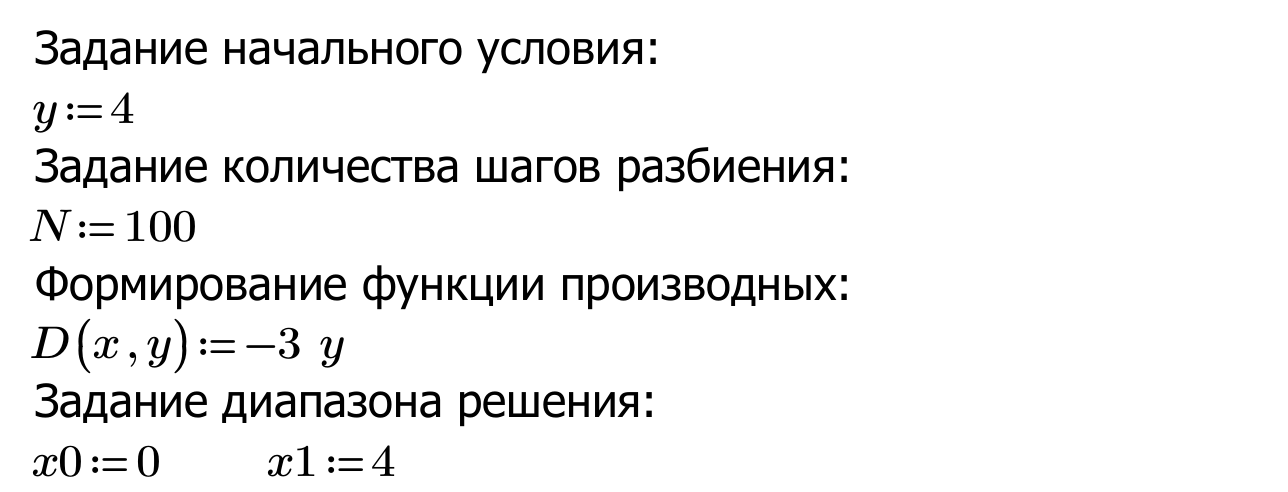
\includegraphics{new-diffeq-1-1.png}
\end{center}
\begin{center}
	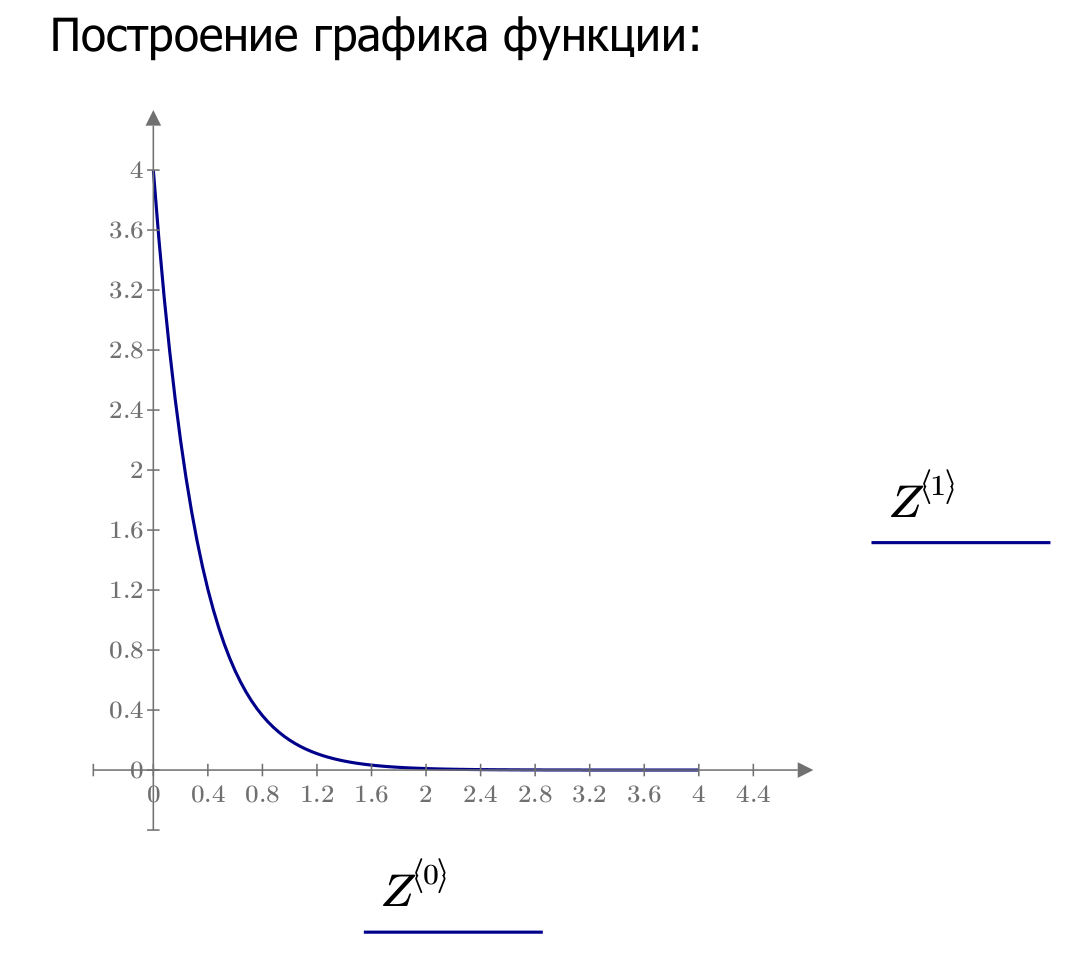
\includegraphics{new-diffeq-1-2.png}
\end{center}

\primer{Решить систему дифференциальных уравнений в интервале [-2; 8] с начальными условиями $y(-2)=1$ и $z(-2)=-10$
	\begin{equation*}
	\begin{cases}
	\dfrac{d y}{d x} - (y-z) \sin(x)=0 \\
	\dfrac{d z}{d x} -\sqrt[3]{y} +z = 0
	\end{cases}
	\end{equation*}
	Результат решения представить графически. }

\begin{center}
	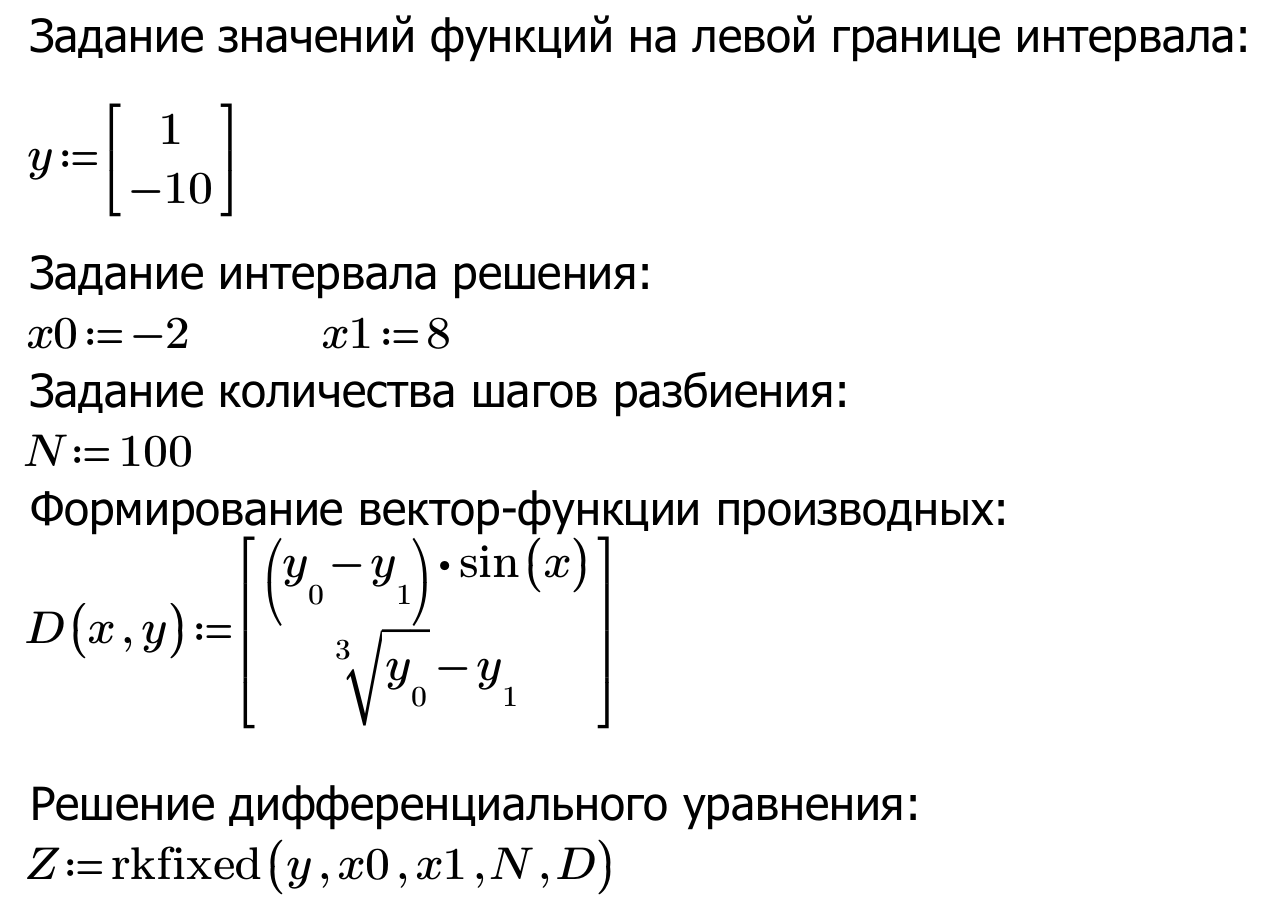
\includegraphics{new-diffeq-2-1.png}
\end{center}

\begin{center}
	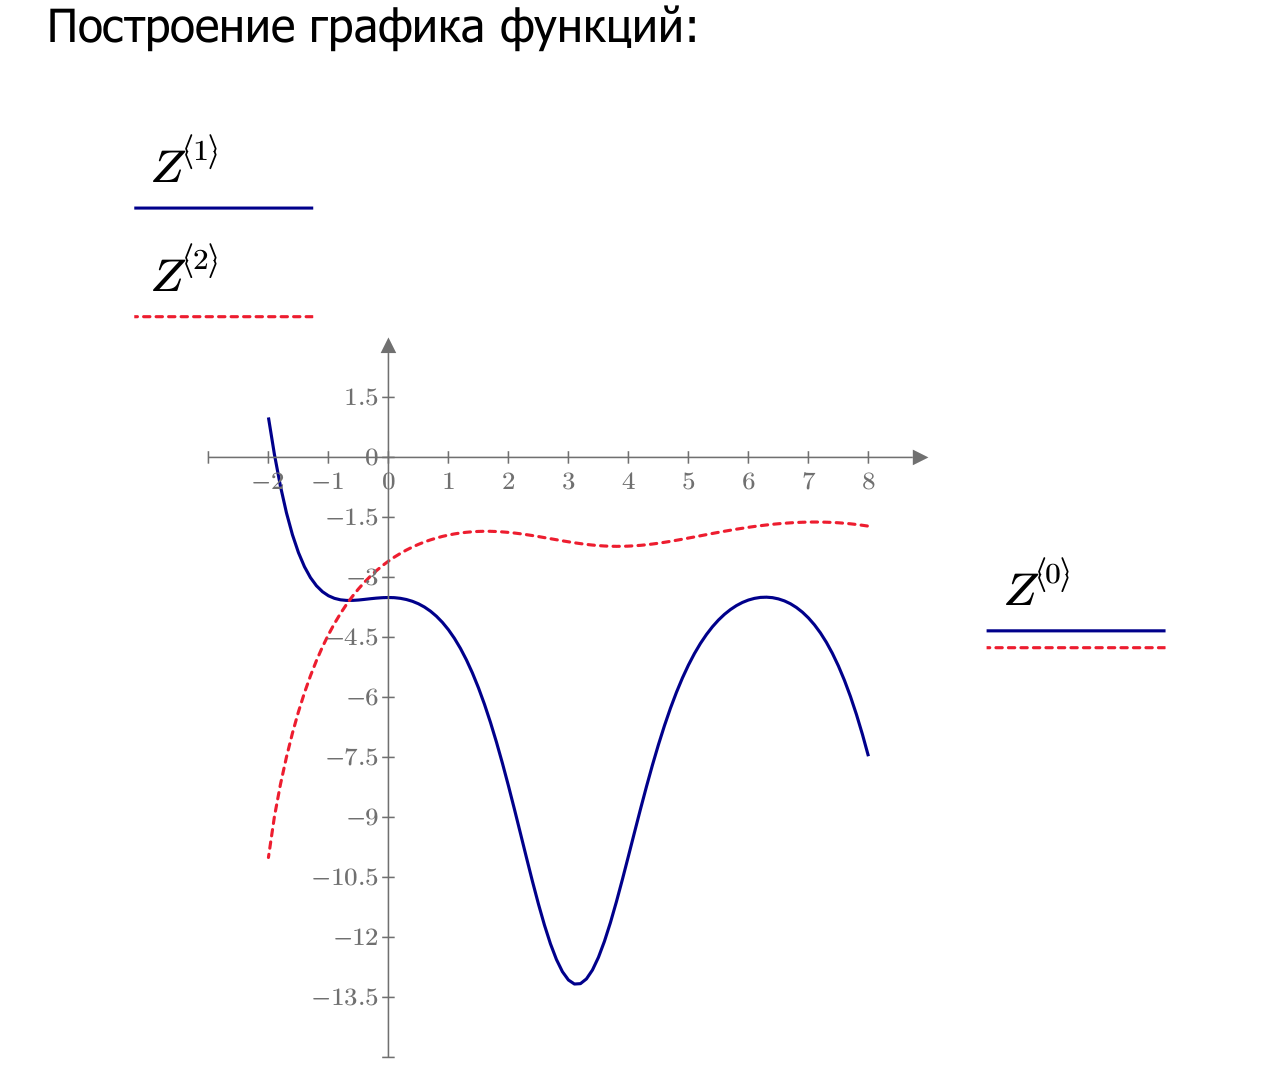
\includegraphics{new-diffeq-2-2.png}
\end{center}

\subsubsection{Дифференциальные уравнения высших порядков}
Если дифференциальные уравнения системы содержат производные от неизвестных функций выше первого порядка, то все уравнения, содержащие такие производные, необходимо преобразовать. Уравнение вида \ref{dif.mdif}, содержащее производные выше первого порядка посредством замены:
\begin{equation}
\begin{gathered}
y_1(x)=y(x),\\ y_2(x)=y^{\prime}(x),\\  ... \\ y_r(x)=y^r(x)
\end{gathered}
\end{equation}
может быть приведено к совокупности уравнений:
\begin{equation}
\begin{gathered}
y_1^{\prime}(x)=y_2(x), \\ y_2^{\prime}(x)=y_3(x), \\ ... \\ y_r^{\prime}(x)=F(x,y_1(x),y_2(x, ... , y_r(x)).
\end{gathered}
\end{equation}
В приведенных выше уравнениях уже нет производных выше первого порядка. Преобразовав подобным образом каждое из уравнений, входящих в исходную систему, получим новую систему с большим количеством неизвестных функций, но с производными только первого порядка. Следовательно, для решения такой системы дифференциальных уравнений можно использовать функцию \mc{rkfixed}, как описано выше.

\primer{Решить систему дифференциальное уравнений второго порядка $y^{''}+y^{'}-y-x=0$ на диапазоне от $x=0$ до $x=3$ при граничных условиях $y(0)=1$, $y'(0)=2$. Построить график функции $y$.}
\begin{center}
	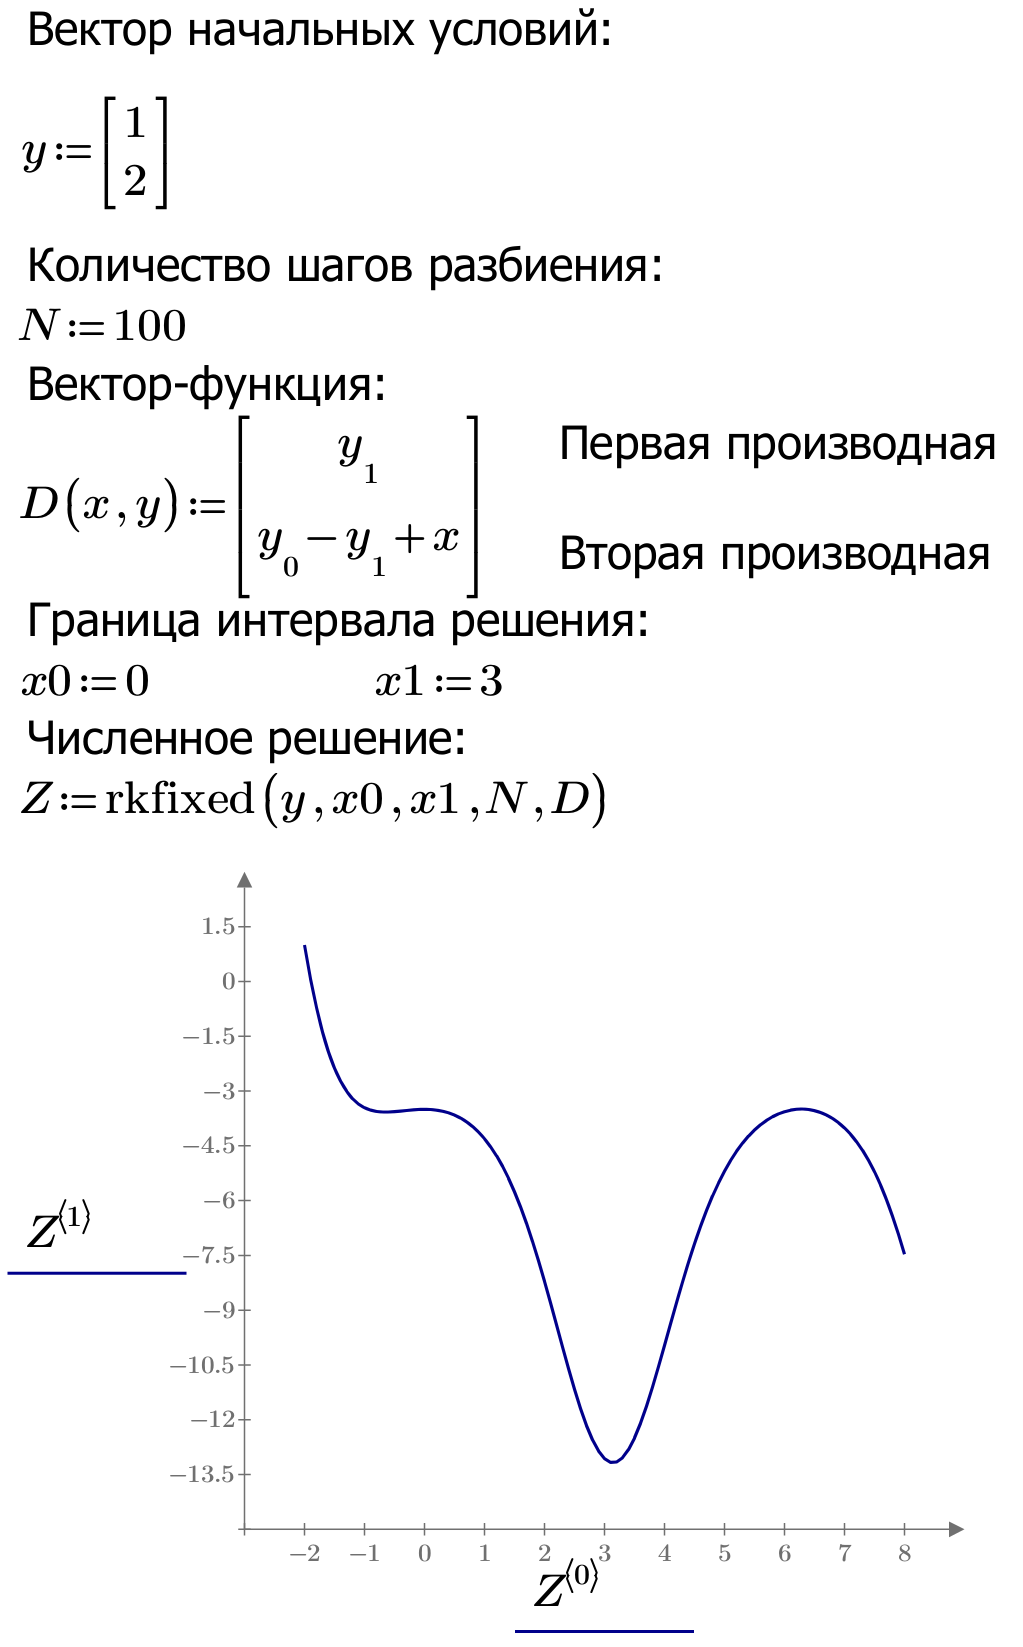
\includegraphics{new-diffeq-3.png}
\end{center}


\primer{С самолета летящего со скоростью 100 $м/с$ сбросили шар, площадь проекции шара 10 $см^2$, масса 1 кг. Построить траекторию движения шара с учетом и без учета сопротивления воздуха за 10 секунд падения. }

Направим ось $x$ параллельно поверхности земли по ходу движения тела, ось $y$ по нормали к поверхности земли вверх. На тело действуют две силы: сила притяжения (направлена вдоль оси $y$ вниз) и сила сопротивления воздуха (действует по обоим осям). силу притяжения можно описать через ускорение свободного падения $g$. Сопротивление воздуха определяется выражением: $F=C_f \frac{\rho \upsilon^2}{2} S$, где $C_f$ --- коэффициент сопротивления, равный 0.49 для сферических тел, $\rho$ --- плотность воздуха равная примерно 1.2 $кг/м^3$, $S$ --- площадь поверхности.

Таким образом необходимо решить систему дифференциальных уравнений:
\begin{equation*}
\begin{cases}
\dfrac{dx}{dt}=\upsilon_x  \\
\dfrac{d \upsilon_x}{dt} = a_x = -\dfrac{F_x}{m}=-\dfrac{C_f}{m} \dfrac{\rho \upsilon_x^2}{2}S \\
\dfrac{dy}{dt}=\upsilon_y  \\
\dfrac{d \upsilon_y}{dt} = a_y = -g+\dfrac{F_y}{m}=-\dfrac{C_f}{m} \dfrac{\rho \upsilon_y^2}{2}S
\end{cases}
\end{equation*}
где, $a$ --- ускорение. Знак "минус" означает, что сила направлена противоположно выбранной оси координат. Граничные условия: $x_0=0~м$ , $\upsilon_{x0}=100~м/с$, $y_0=0~ м$, $\upsilon_{y0}=0~ м/с$.

\begin{center}
	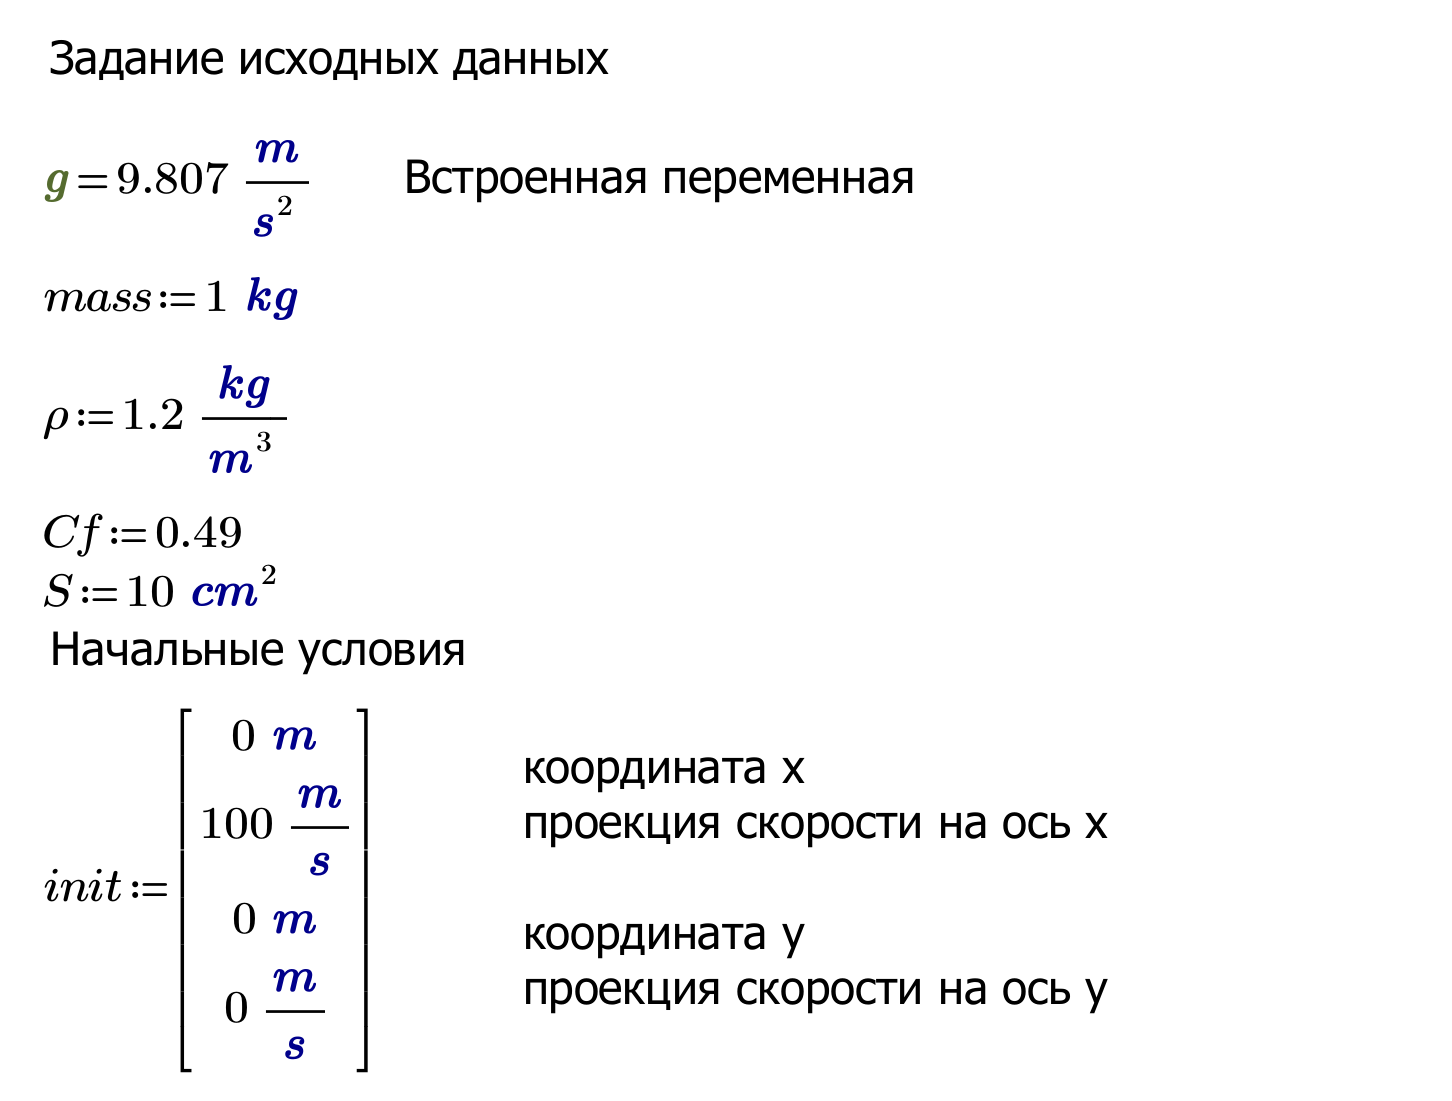
\includegraphics{new-diffeq-4-1.png}
\end{center}
\begin{center}
	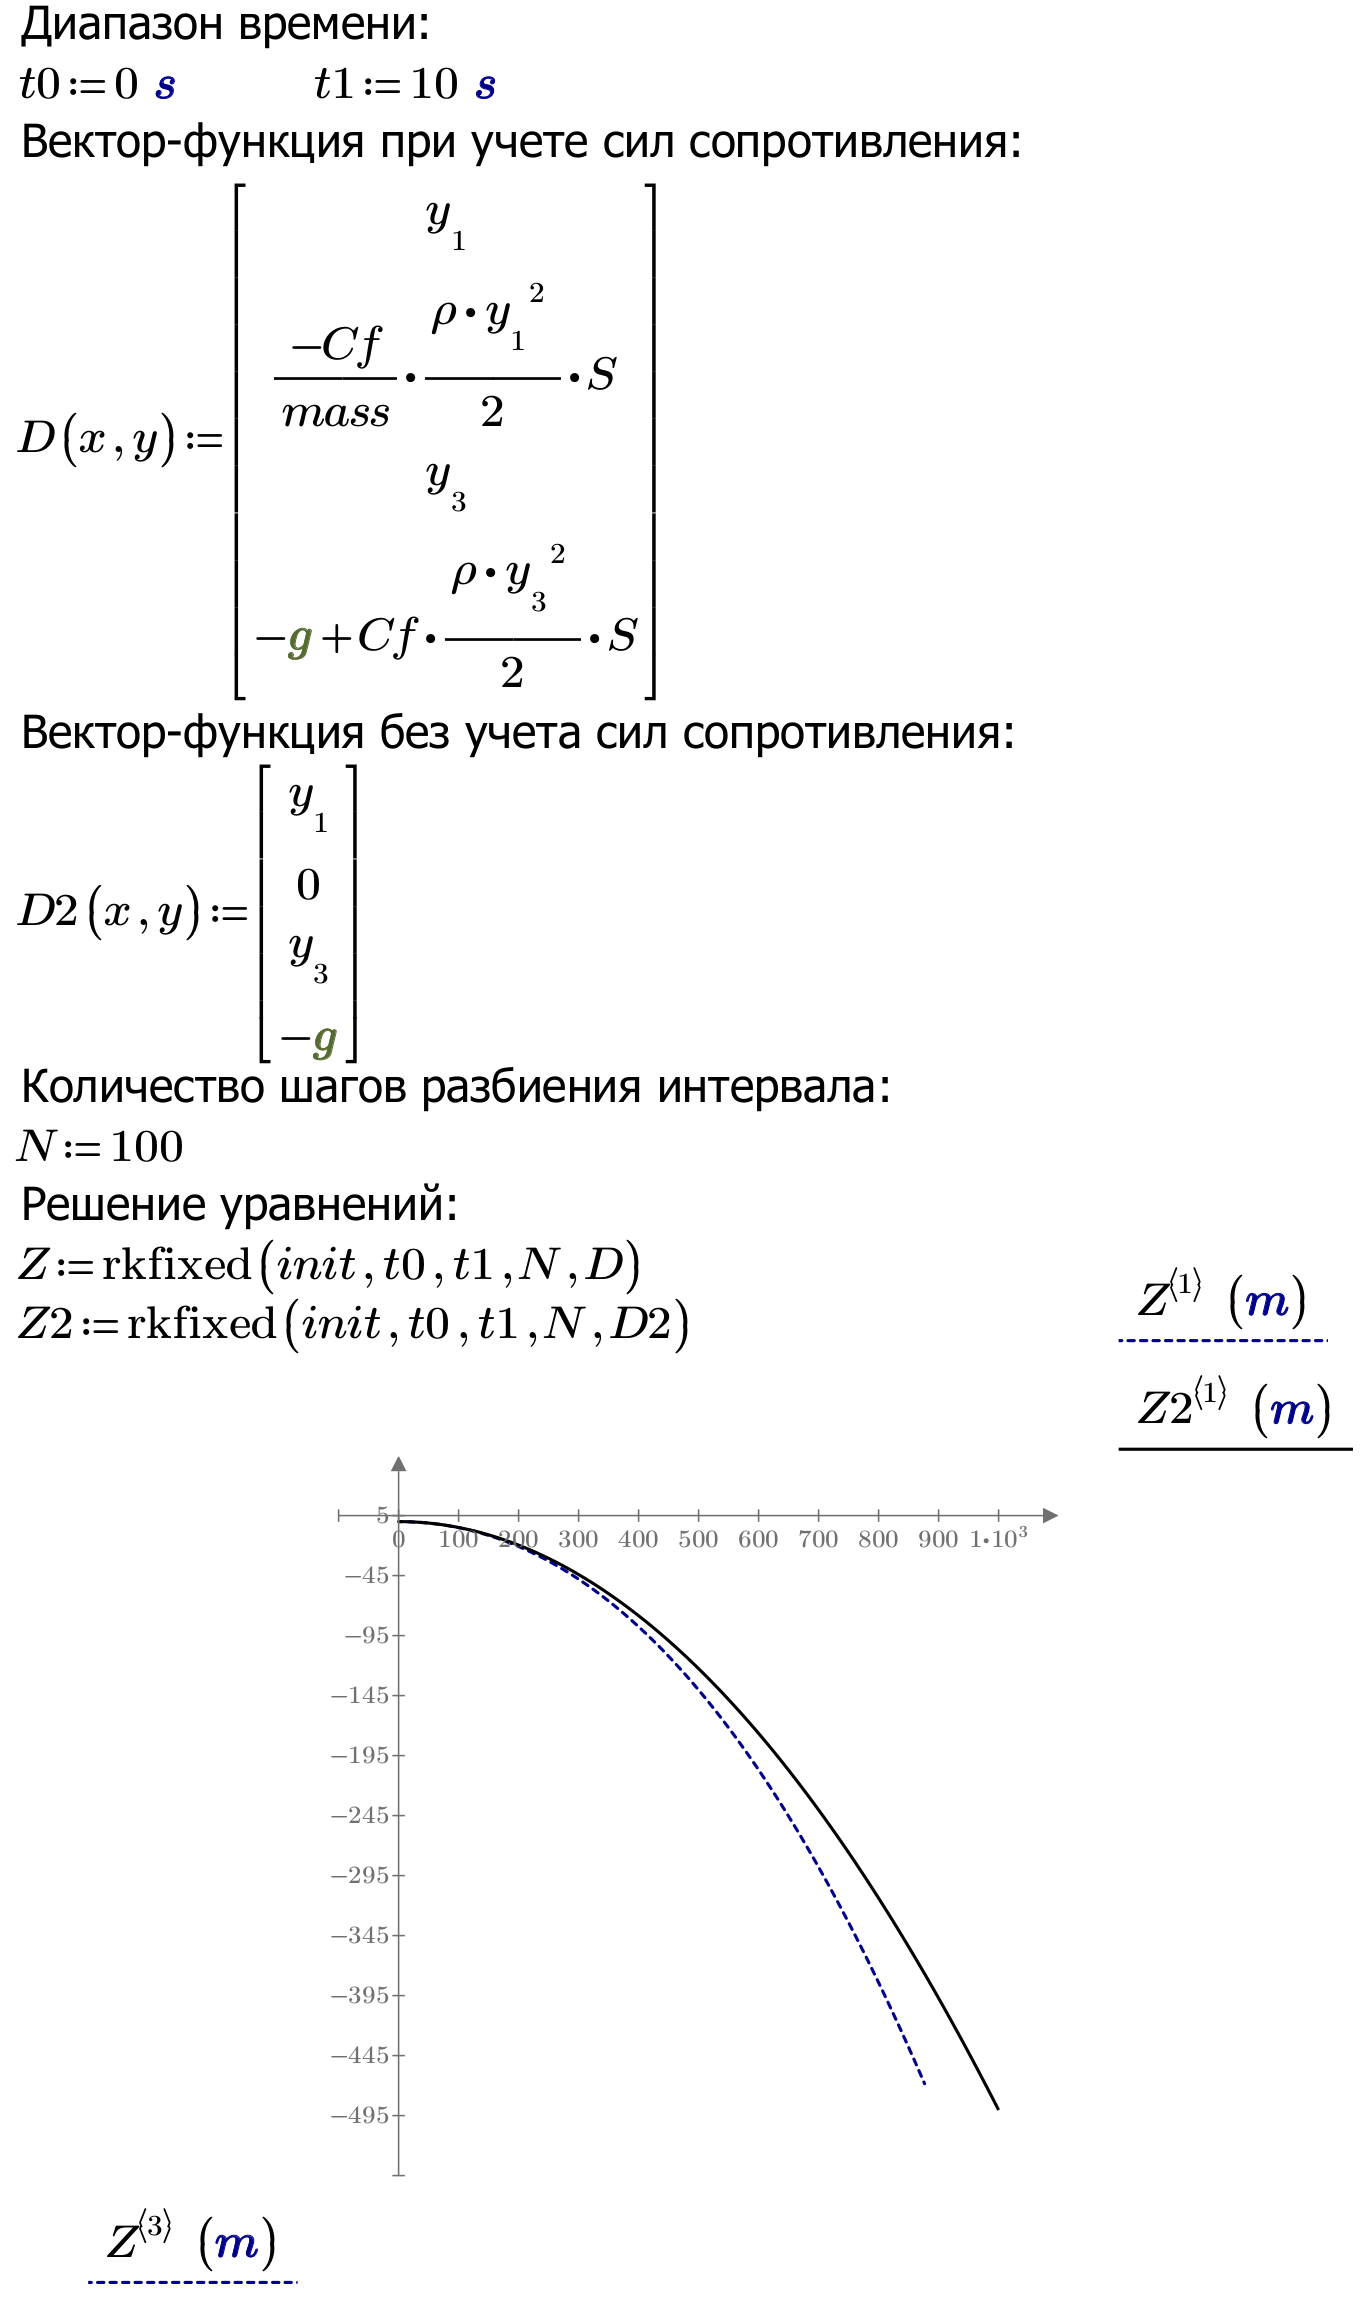
\includegraphics{new-diffeq-4-2.png}
\end{center}
\subsubsection*{Решение краевых задач}

Краевые задачи отличаются от задач Коши тем, что начальные условия для них задаются на обеих границах интервала поиска решений. Краевая форма для дифференциальных уравнений и их систем используется в основном в физике и технике в тех случаях, когда определить все начальные значения на одной границе интервала невозможно. 

Найти решение для заданных таким образом дифференциальных уравнений возможно только на основе алгоритма, в котором многократно решается задача Коши. Суть этого алгоритма заключается в подборе (естественно, направленном) недостающих параметров на одной из границ интервала, исходя из того условия, что соответствующие решения полученной задачи Коши в противоположной точке интервала должны совпадать с исходными краевыми условиями с определенным уровнем точности.

Для решения краевых задач в Mathcad имеется встроенная функция \mc{sbval(z,t0,t1,D,load,score)}. Данная функция требует определения следующих параметров:
\begin{itemize}[label={}]
	\item \mc{z} --- вектор начальных приближений, в котором необходимо определить исходные значения для недостающих на левой границе условий. Выбор начального приближения оказывает влияние на сходимость и время поиска решения;
	\item \mc{t0} и \mc{t1} --- начальная и конечная точки интервала, на котором ищется решение системы дифференциальных уравнений;
	\item \mc{D(x,y)} --- вектор-функция, описывающая дифференциальное уравнение или систему уравнений. Задается аналогично рассмотренной ранее встроенной функции \mc{rk\-fix\-ed};
	\item \mc{load(t0,z)} --- векторная функция двух переменных, описывающая значение функции на левой границе интервала. Представляет собой вектор из \mc{N} элементов (\mc{N} соответствует количеству уравнений системы), каждый из которых является значением соответствующей функции вектора \mc{y} в точке \mc{t0}. Если начальное значение некоторой функции неизвестно, в качестве элемента \mc{load} следует использовать величину из вектора приближений \mc{z};
	\item \mc{score(t1,y)} --- векторная функция, служащая для задания правых граничных значений. Элементы вектора \mc{score} должны быть заданы как разности известных начальных значений в точке \mc{t1} и соответствующих им значений функций \mc{y}, возвращаемых функцией \mc{sbval}. Алгоритм, лежащий в основе функции \mc{sbval}, использует текущие величины \mc{score} в качестве меры точности подобранных приближений. 
\end{itemize}

Результатом работы функции \mc{sbval} является вектор с найденными значениями начальных условий, недостающих для представления системы дифференциальных уравнений в форме задачи Коши. Определив начальные условия можно решить данную систему дифференциальных уравнений используя встроенную функцию \mc{rkfixed}.  При этом  в качестве  ее параметра \mc{у0} можно использовать уже определенную выше функцию \mc{load} (обозначив вектор результата как \mc{z}).

\primer{Решить краевую задачу для систем дифференциальных уравнений в интервале [0; 2] с граничными условаиями $y(0)=3$ $z(2)=1.6$:
	\begin{equation*}
	\begin{cases}
	\dfrac{d y}{d x} + 3 x y -z =0 \\
	\sqrt[3]{z} -y - \dfrac{d z}{d x}  = 0
	\end{cases}
	\end{equation*}
	Результат решения построить графически.
}
\begin{center}
	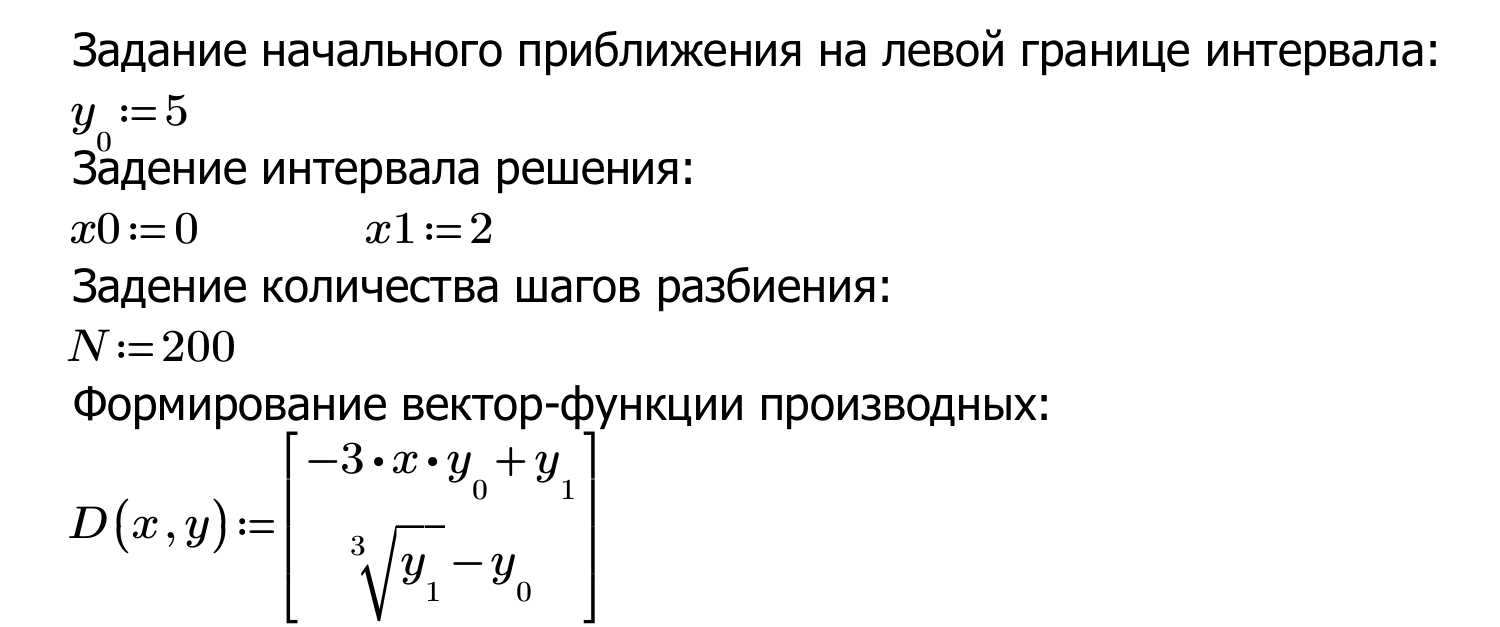
\includegraphics{new-diffeq-5-1.png}
\end{center}

\begin{center}
	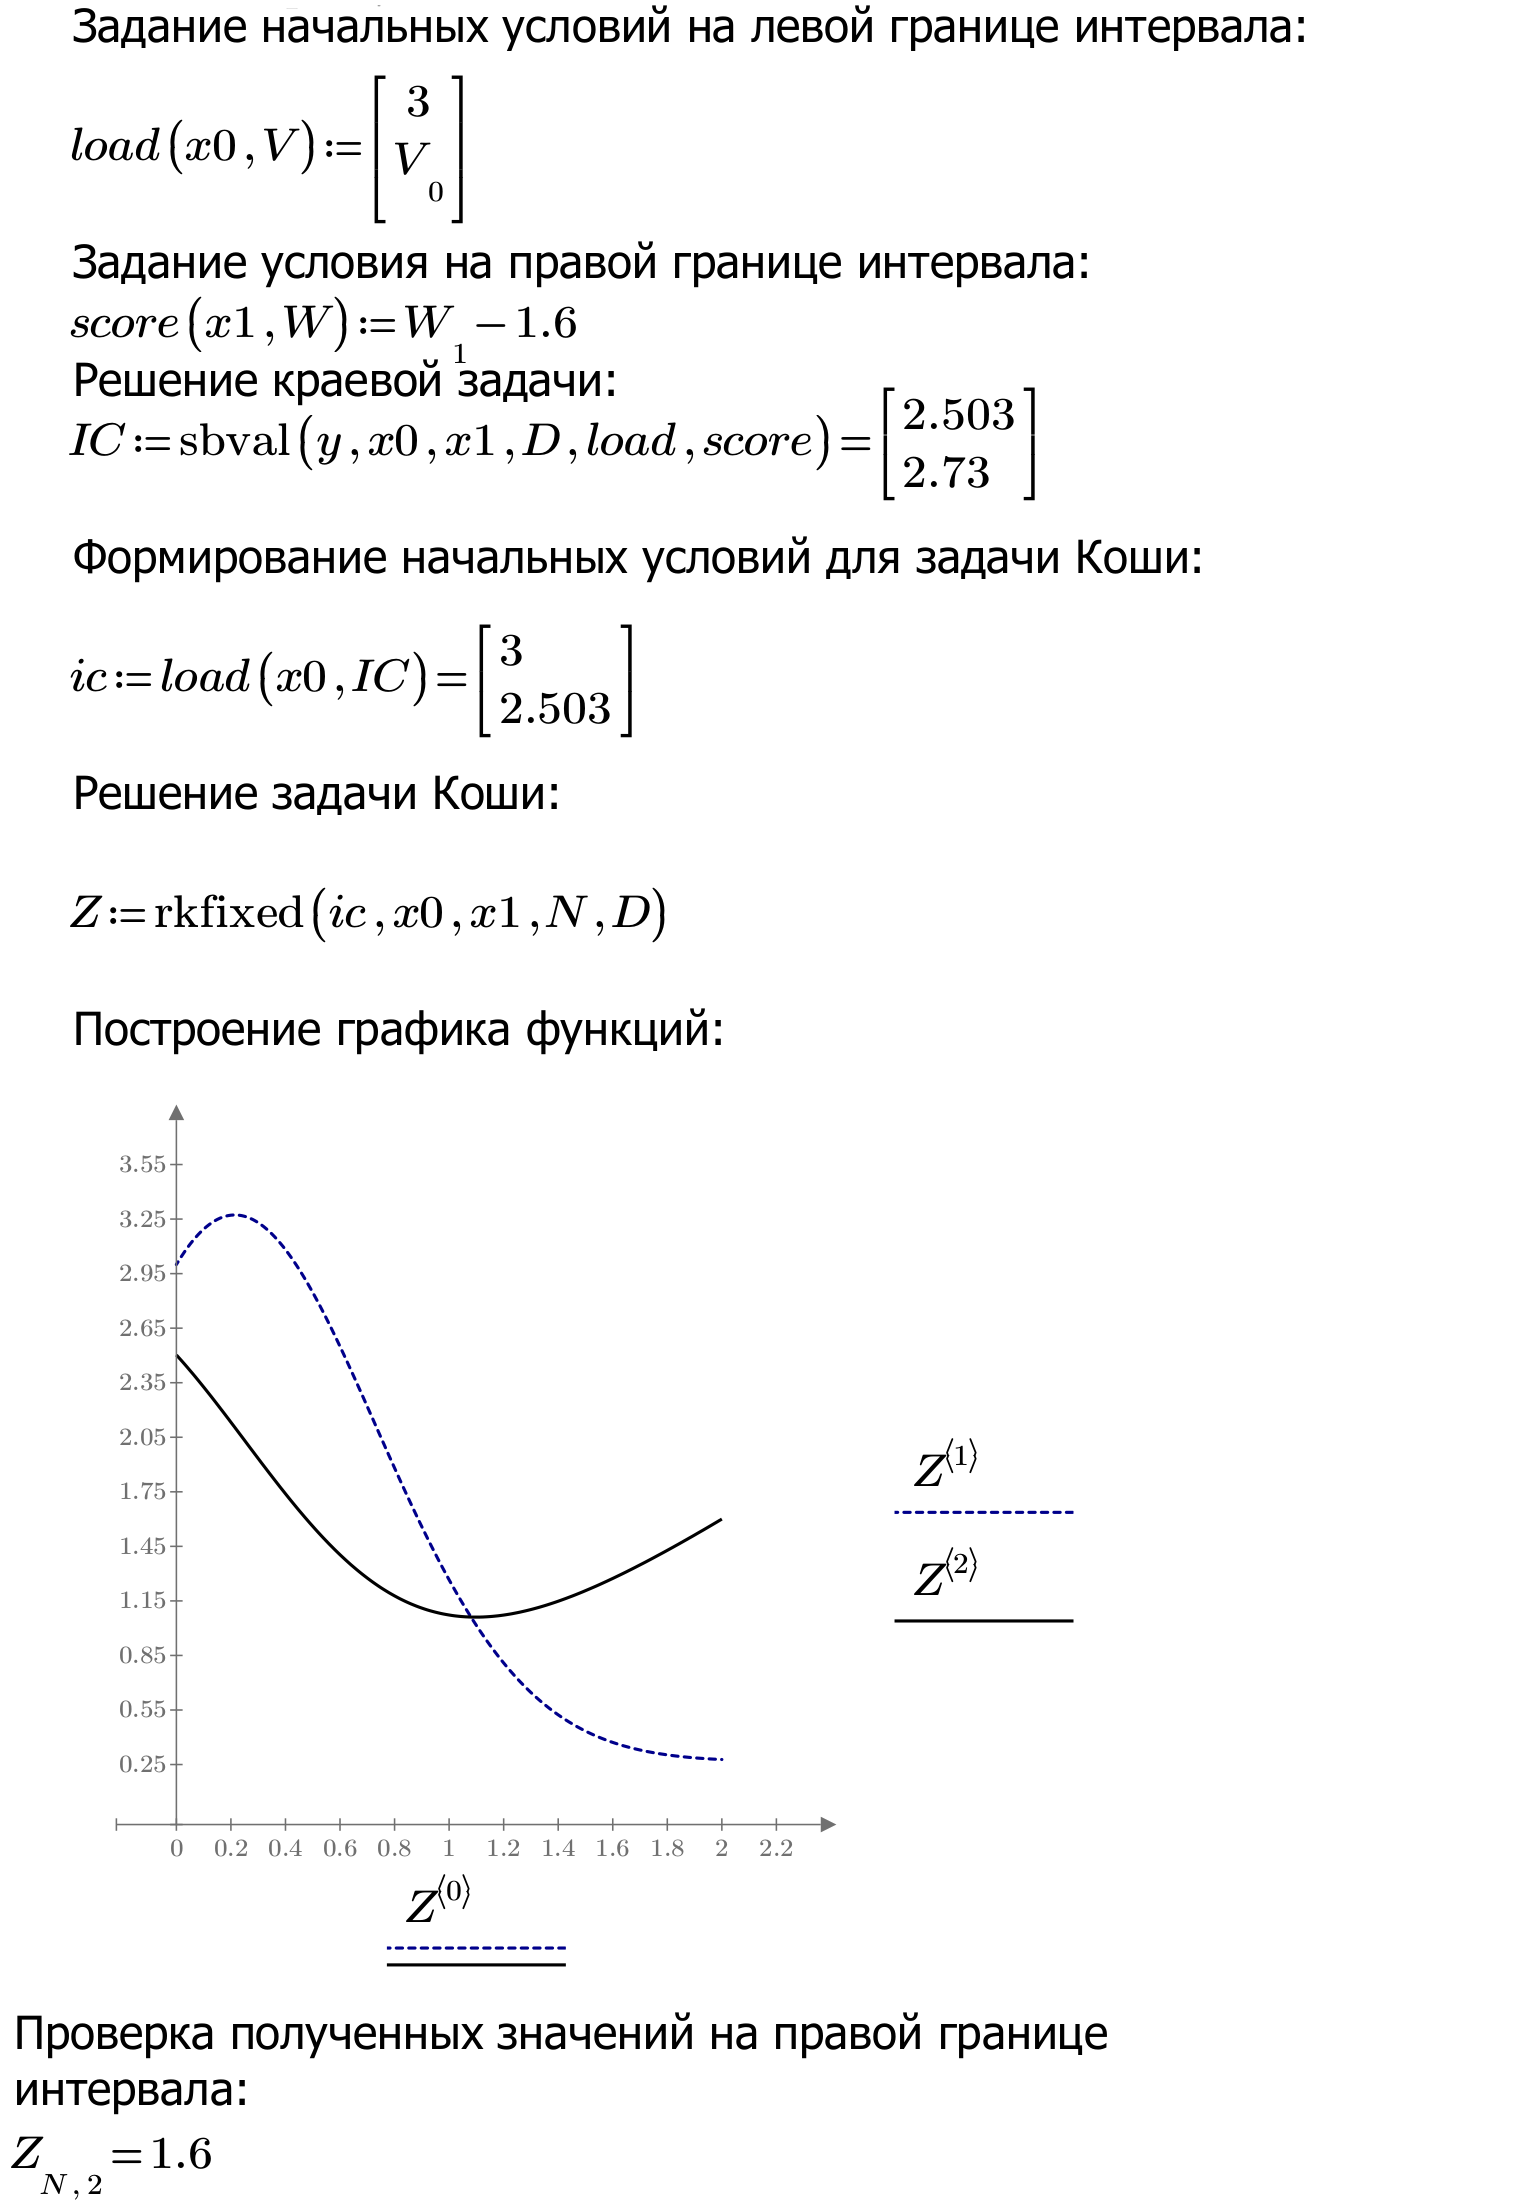
\includegraphics{new-diffeq-5-2.png}
\end{center}

\subsubsection*{Примеры составления дифференциальных уравнений}
\primer{ В сосуд объемом $V\ м^3$, содержащий чистую воду, подведено две трубы. По трубам поступает $j_1$ и $j_2 \frac{м^3}{ч}$ раствора соли, концентрацией $c_1$ и $c_2 \frac{кг}{м^3}$ соответственно. Раствор мгновенно перемешивается, что соответствует модели идеального смешения. Излишки смеси вытекают в канализацию. Необходимо составить математическую модель для описания массы соли находящейся в сосуде.}

При составлении дифференциального уравнения необходимо учитывать входящие и выходящие потоки массы. Входящие потоки увеличивают массу соли в сосуде, и записываются в дифференциальное уравнение со знаком <<+>>, выходящие --- соответственно со знаком <<$-$>>. Масса соли, приходящая с первым потоком равна $j_1 c_1$, со вторым --- $j_2 c_2$. Выходящий поток имеет ту же концентрацию, что и в самом сосуде и может быть выражена через массу соли в сосуде и его объем $c=\frac{m}{V}$.

Соответственно уравнение изменения массы по времени будет записано в виде:
\begin{equation}
\dfrac{d m}{d \tau} = j_1 c_1 + j_2 c_2 - (j_1 + j_2 ) \dfrac{m}{V}
\end{equation}

Дифференциальное уравнение дополняем начальными условиями: в начальный момент времени в сосуде содержится чистая вода, соответственно $m(0)=0.$

\primer{В баке цилиндрической формы (высота $h$ м, диаметр $D$ см) проделали круглое отверстие диаметром $d$~см. Бак доверху наполнили водой закрыв отверстие. Определить, через какое время после открытия отверстия в баке останется $V_k$ литров воды? }

Усредненная по поверхности отверстия скорость истечения равна:
\begin{equation}
\bar{w}=\phi \sqrt{2gH}
\end{equation} 
где $\phi$ --- коэффициент скорости, для отверстий в тонкой стенке равный 0.97, $H$ --- высота столба жидкости в резервуаре над отверстием.

Расход жидкости можно записать умножая скорость истечения на площадь отверстия:
\begin{equation}
\dfrac{d V}{d \tau} = - S  \varepsilon \bar{w}= -\dfrac{\pi d^2}{4} \varepsilon  \phi \sqrt{2gH}
\end{equation}
где $\varepsilon$ --- коэффициент сжатия струи, для отверстий в тонкой стенке равный 0.64. Знак  <<$-$>> в дифференциальном уравнении показывает,  что объем воды в резервуаре течением времени уменьшается. 

Дифференциальное уравнение дополняем начальным условием: в начальный момент времени резервуар полный, следовательно $V(0)=\frac{h \pi D^2}{4}$


\primer{В комнату объемом $V$ $\text{м}^3$ и температурой воздуха $T_{air}$ $\mathrm{C^\circ}$ внесли разогретый до $T$ $\mathrm{C^\circ}$ предмет массой $m$ кг, теплоемкость материала $c_p$ ${\frac{Дж} {кг С^\circ}}$. Считая комнату плотностью изолированной, и принимая условие высокой теплопроводности как тела, так и воздуха, определить температуру воздуха через $n$ часов при условии что коэффициент теплоотдачи равен $K$ ${\frac{Вт}{м^2 К}}$.  }

Уравнение теплопередачи имеет вид:
\begin{equation}
q=K F \Delta T
\end{equation}
где $q$ --- тепловой поток, $F$ --- поверхность теплопередачи, $\Delta T$ --- разница температур двух тел. Изменение температуры тела можно определить по количеству тепла, принятого или отданного телом:
\begin{equation}
\dfrac{d T}{d \tau}=\dfrac{q}{c m} = \dfrac{K F \Delta T}{c m}
\end{equation}
где $c$ --- теплоемкость тела, $m$ --- масса тела.
Теперь можно записать систему уравнений:
\begin{equation}
\begin{cases}
\dfrac{d T_1}{d \tau} = \dfrac{K F (T_2-T_1)}{c_1 m_1} \\
\dfrac{d T_2}{d \tau} = \dfrac{K F (T_1-T_2)}{c_2 m_2}
\end{cases}
\end{equation}
индексами 1 и 2 обозначены соответственно разогретый предмет и окружающий воздух. В первом уравнении знак <<->> означает, что тело отдает тепло, соответственно температура тела уменьшается. В качестве начального условия необходимо задать температуры воздуха и тела в начальный момент времени $T_1(0) = T$, $T_2(0) = T_{air}$

\primer{Толщина плоской стенки теплоизоляции $l см$, теплопроводность стенки $\lambda \dfrac{Вт} {м \cdot гр}$. Температура горячей стороны теплоизоляции $T_h \mathrm{C^\circ}$. Определить температуру с холодной стороны, если тепловой поток равен $q \frac{Вт}{м^2}$}.

Распределение температуры вдоль стенки теплоизоляции можно определить по закону Фурье:
\begin{equation}
q=-\lambda \dfrac{d T}{d x}
\end{equation} 
В случае постоянства теплового потока $q$ и теплопроводности $\lambda$ можно записать дифференциальное уравнение:
\begin{equation}
\dfrac{d T}{d x} =- \dfrac{q}{\lambda}
\end{equation}
Аналитическое решение уравнения, с учетом начального условия $T(0) = T_h$, будет иметь вид:
\begin{equation}
T = T_h - \dfrac{q x}{\lambda}
\end{equation}

Вопросы для самоконтроля:
\begin{enumerate}
	\item Что такое обыкновенное дифференциальное уравнение и чем определяется его порядок?
	\item Какие данные необходимы для поиска решения дифференциального уравнения?
	\item Что является решением дифференциального уравнения?
	\item Что такое задача Коши?
	\item Что такое краевая задача?
	\item Что влияет на точность и трудоемкость численного решения системы дифференциальных уравнений?
\end{enumerate}

\subsubsection*{Пример задания}
\begin{enumerate}
	\item Решить численно дифференциальное уравнение $\dfrac{dy}{dx}=\sqrt{\dfrac{4x}{y}}$ с начальными значениями $y(     2)=     1$ на интервале от $x=     2$ до $x=    11$. Построить график функции.\item Решить численно систему дифференциальных уравнений:
	\begin{equation*}
	\left\{
	\begin{gathered}
	\dfrac{dy}{dx}=x-2y                  \\
	\dfrac{dz}{dx}=\dfrac{x^2}{y}        
	\end{gathered}
	\right.
	\end{equation*}
	на интервале от $x= 7$ от $x=17$ с граничными условиями: $y( 7)=1.43$, $z( 7)=2.12$. Построить график функции. 
	\item Решить численно систему дифференциальных уравнений:
	\begin{equation*}
	\left\{
	\begin{gathered}
	\dfrac{dy}{dx}=\sqrt{|x+y+z|}\\
	\dfrac{dz}{dx}=\dfrac{x^{0.8}}{5+sin(y)}
	\end{gathered}
	\right.
	\end{equation*}
	на интервале от $x= 1$ от $x= 5$ с граничными условиями: $y( 1)=4.24$, $z( 5)=3.72$.  Построить график функции. 
	\item  В баке находится 223.2 л раствора, содержащего 30.95 кг соли. В бак непрерывно подается вода (расход воды 1.1 л/мин), которая перемешивается с имеющимся раствором. Смесь вытекает с тем же расходом. Записать дифференциальное уравнения изменения массы соли. Построить график зависимости концентрации соли от времени. Определить какое количество соли в баке останется через  117 минут?
	
	\item  При комнатной температуре 20$^\circ\mathrm{C}$ в печь поместили заготовку массой 5.6 кг и поверхностью 2.9 $\text{м}^2$, после включения температура воздуха в печи равномерно увеличивалась на 4.1 градуса в минуту. Плотность материала заготовки --- 4206.3 $\text{кг}/\text{м}^\mathrm{3}$, теплоемкость --- 915.4 $\frac{\text{Дж}}{\text{кг} \cdot град}$. Коэффициент теплопередачи между воздухом и металлом равен   463 $\frac{Вт}{м^2 град.}$. Определить через какое время металл нагреется до температуры   511 градусов.
\end{enumerate}
